\chapter{Implementation}
\label{chap:Chapter 4 title}
\section*{Introduction}

The implementation chapter is a crucial step in our project. In this chapter, we will present in detail the various steps we followed to implement our solution. Overall, this implementation chapter will allow us to document in a detailed and transparent manner the process of executing our project. It will highlight the efforts made, the choices made, and the results obtained.

\pagebreak

\section{Creating a GitLab Template for Kepler}

To successfully integrate Kepler with our GitLab CI pipeline and ensure a seamless, efficient, and automated workflow, we followed a series of steps that included configuring the necessary environments, creating precise configuration files, and integrating essential monitoring tools
\subsection*{Configuration of the Environment}

The initial step was to set up the execution environment for GitLab CI. We configured the runners, which are the virtual machines or containers responsible for executing the CI jobs. It was crucial to ensure that all dependencies required to run Kepler, Prometheus, and Grafana were installed on these runners.

\subsection*{Creation of the CI Configuration File}

We added a \texttt{template-ci-kepler.yml} file. This file plays a 
role as it defines the various stages of the CI pipeline and specifies the actions required to integrate Kepler into our CI process. By using this configuration file, we were able to clearly and systematically outline the tasks necessary for seamless integration into our pipeline.

 \begin{figure}[H]
    \centering
    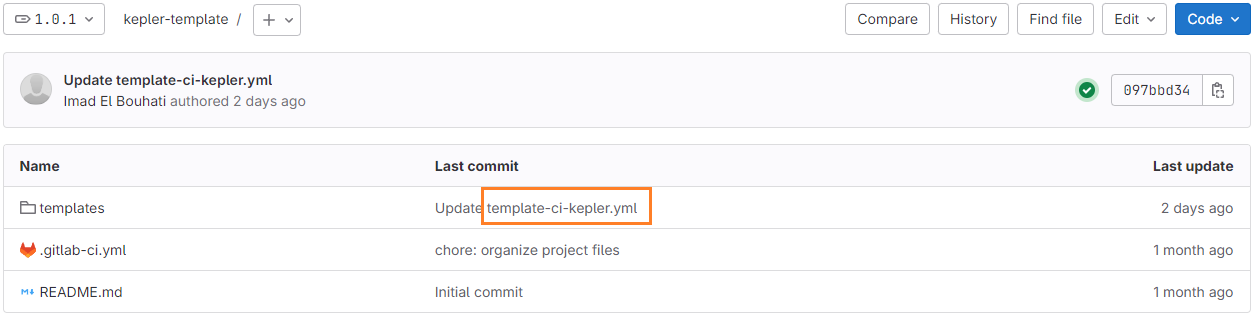
\includegraphics[width=19cm]{Figures/kepler-template-gitlab.png}
    \caption{Kepler template repository}
\end{figure}

\subsection{Integration of the Kepler Template}

After creating the template, it can be used and integrated directly into a project. To achieve this, a few lines must be added to the \texttt{.gitlab-ci.yml} file.

First, we add the \texttt{include} directive followed by the path to our directory containing the Kepler template into an existing pipeline.

\begin{figure}[H]
  \centering
  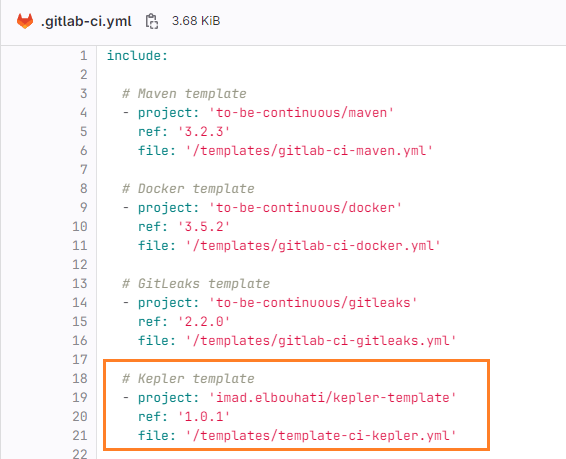
\includegraphics[width=13cm]{Figures/kepler-template-integration.png}
  \caption{Integration of the Kepler template}
\end{figure}

Next, we specify the stage name as \texttt{"deploy"}.

\begin{figure}[H]
  \centering
  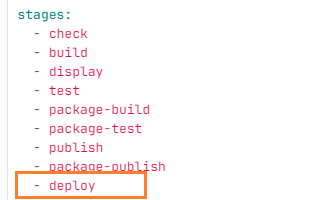
\includegraphics[width=10cm]{Figures/deploy-kepler-stage.png}
  \caption{Stage \texttt{"deploy"}}
\end{figure}

We define the following variables for the deployment:

\begin{itemize}
    \item \texttt{HELM\_RELEASE\_NAME} as the name of our Helm release.
    \item \texttt{HELM\_NAMESPACE} as the namespace for our Helm deployment.
    \item \texttt{KUBECONFIG\_CONTENT} to store cluster authentication information for kubectl.
\end{itemize}

\begin{figure}[H]
  \centering
  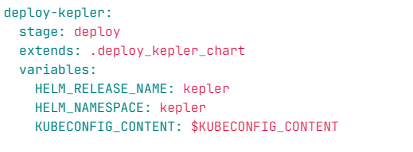
\includegraphics[width=0.8\textwidth]{Figures/deployment-variable.png}
  \caption{Deployment variables for Kepler}
\end{figure}

This configuration allows us to include the steps for deploying Kepler in our CI/CD pipeline using Helm and Kubernetes.


\section{Deploying Prometheus \& Grafana on Kubernetes}

\section{Configuring Rules and Alerts in Prometheus}
\subsection{Setting Up Alerting Rules}
\subsection{Configuring Alerts in Prometheus}

\section{Slack Integration with Prometheus Alerts}
\subsection{Configuring Slack for Prometheus Alerts}
\subsection{Testing Slack Integration}

\section{Conclusion}







\newpage

\section*{Conclusion}

Lorem ipsum dolor sit amet, consectetur adipiscing elit. Praesent nec dapibus justo. Donec sagittis vulputate ante sed porttitor. Suspendisse sit amet nisl massa. Curabitur nec nisl condimentum, egestas ex vitae, dapibus enim. Etiam iaculis, erat faucibus pellentesque sagittis, nisi justo sollicitudin nibh, et condimentum augue massa non turpis. Proin commodo enim fermentum suscipit condimentum. Maecenas molestie, dui nec vestibulum rhoncus, arcu nisl faucibus neque, a ornare nisi massa ac eros. Aenean id velit sit amet lacus mattis varius. Donec fringilla massa sed nisi eleifend, a aliquet mi tempus. Nunc posuere euismod est, nec tristique augue lobortis non. Sed sodales sem ut metus tempus ullamcorper.

\pagebreak